\documentclass[11pt,letterpaper]{article}

\usepackage{hyperref}
\usepackage{graphicx}
\usepackage{fancybox}
\usepackage[utf8]{inputenc}
\usepackage{epsfig,graphicx}
\usepackage{multicol,pst-plot}
\usepackage{pstricks}
\usepackage{amsmath}
\usepackage{amsfonts}
\usepackage{amssymb}
\usepackage{eucal}
\usepackage{upgreek}
\usepackage[left=2cm,right=2cm,top=2cm,bottom=1cm]{geometry}
\usepackage{tcolorbox}
\usepackage{import}
\pagestyle{empty}
\DeclareMathOperator{\tr}{Tr}
\renewcommand{\sp}[1]{$${\begin{split}#1\end{split}}$$}

\usepackage{lipsum}
\usepackage{mdframed}
\usepackage{listings}
\usepackage{color}

% Margins
% \topmargin=-0.45in
\evensidemargin=0in
\oddsidemargin=0in
\textwidth=6.5in
\textheight=9.0in
\headsep=0.25in

 % The problem environment introduced.                                     
\newenvironment{problem}[2][Problem]                                  
        {\begin{tcolorbox}[colback=white,colframe=gray!50,title=#1 #2]}
        {\end{tcolorbox}}
        % {\begin{mdframed}[backgroundcolor=gray!20] \textbf{#1 #2} \\}
        % {\end{mdframed}}
% Define solution environment
\newenvironment{solution}                      
        {\begin{mdframed}\textit{Solution:} \\}
        {\end{mdframed}}
% Define an environments for proofs
\newenvironment{myproof} 
        {\textit{Proof:}}                                   
        {\begin{flushright} Q.E.D. \end{flushright}}
% Define a theorem environment and a notation one too
\newenvironment{mytheorem}                    
        {\begin{mdframed}\textbf{Theorem:} \\}
        {\end{mdframed}}
\newenvironment{notation}                      
        {\begin{mdframed}\textit{Notation:} \\}
        {\end{mdframed}}
% A new example wouldnt so any harm either...  
\newenvironment{example}                             
        {\textit{Example:}\\}
	{}
%I should be ashamed to forget the definition environment
\newenvironment{definition}
	{\begin{mdframed}$\underline{\textit{Def}^\textit{n}:} $\\}
	{\end{mdframed}}
%Corollary envvvvvvvvv
\newenvironment{corollary}
	{\textbf{Corrolary:}\\}

\pagestyle{empty}

\begin{document}

\begin{center}
  \Huge{Discrete Math Notes}\\
  \vspace{0.25cm}
  \small{Gurmukh Singh}
\end{center}

\vspace{-1.75cm}

\begin{flushright}
  Instructor: \\ Dr. Sanjay Kumar
\end{flushright}

\vspace{-1.3cm}

\begin{flushleft}
  B.Tech. CSE
\end{flushleft}

\rule{15.5cm}{0.1mm}%{\linewidth}{0.1mm}

% Optional TOC
\tableofcontents
\pagebreak

%--Paper--

\section{UNIT 1}
\subsection{Set Theory}
Schaum series- Lipscitz

\subsubsection{Sets}
Sets are \underline{well defined} collection of mathematical objects.

\begin{example}
  The collection of best mathematicians in the world is not a set as there is no fixed criteria for being the best mathematicians.
\end{example}

Notation: Sets are denoted by capital letters such as $A,B,X,Y$. \\
the elements are denoted by small letters such as $a,b,x,y$. 

\begin{definition}
  A set $A$ is called to be a subset of $B$ iff
  \[
    a \in A \implies a \in B
  \]
  It is denoted by $A \subseteq B$.
\end{definition}

\subsubsection{Empty and Universal set}
\begin{definition}
  An empty set is a set which contains no elements. It is either denoted by empty braces or the greek letter $\phi$.
\end{definition}
\begin{definition}
  A Universal set is a set which contains all the elements (in the context). 
\end{definition}
\begin{definition}
  A set which contains only one element is called a singleton set. \\ 
  for example: $\{5\}$.
\end{definition}

Note: \\
for any set $A$, $\phi$ and $A$ are always subsets called improper subsets. 

\subsubsection{Power Set}
\begin{definition}
  A power set of a set is the collection of all the subsets of $A$. It is denotes by $2^A$.
\end{definition}

\subsection{Representation of Sets}
There are 2 ways to represent sets:
\begin{enumerate}
  \item Set builder form 
  \item Roaster form
\end{enumerate}

\subsubsection{Set builder form}
\begin{definition}
  It is based on the unique property of the collection. The iterator is set and a property is defined in curly braces
\end{definition}
\begin{example}
  \[
    A = \{x: x = 2y, y \in \mathbb{Z}\}
  \]
  \begin{center}
    OR
  \end{center}
  \[
    A = \{2x: x \in \mathbb{Z}\}
  \]
\end{example}

\subsubsection{Roaster form}
\begin{definition}
  In this representation we list the elements in curly braces seperated by commas. 
\end{definition}
\begin{example}
  \[
    A = \{\dots,-4,-2,0,2,4,\dots\}
  \]
\end{example}

\subsection{Operations on sets}
We have defined the following functions on sets 
\begin{enumerate}
  \item Union
  \item Intersection
  \item Difference
  \item Symmetric Difference
\end{enumerate}

\subsubsection{Union of Sets($\cup$)}
\begin{definition}
  Collection of all the elements of the sets
\end{definition}
\begin{example}
  \[
    A\cup B= \{x: x\in A \text{ or } x\in B\}
  \]
\end{example}

\subsubsection{Intersection of Sets($\cap$)}
\begin{definition}
  Collection of all the elements in both the sets
\end{definition}
\begin{example}
  \[
    A\cap B= \{x: x\in A \text{ and } x\in B\}
  \]
\end{example}

\subsubsection{Difference of Sets(-)}
\begin{definition}
  Collection of all the elements one set but not the other
\end{definition}
\begin{example}
  \[
    A-B= \{x: x\in A \text{ and } x\not\in B\}
  \]
\end{example}

\subsubsection{Symmetric difference of Sets($\Delta$)}
\begin{definition}
  Collection of all the elements which exist in exactly one of the sets
\end{definition}
\begin{example}
  \[
    A\Delta B= (A-B) \cup (B-A) = (A\cup B) - (A\cap B)
  \]
\end{example}

\subsection{Venn diagram}
A pictorial representation of sets is called a venn diagram\\
\begin{center}
  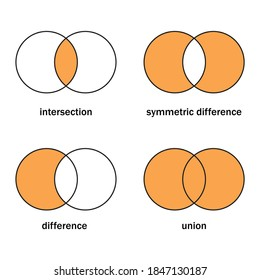
\includegraphics[width=0.5\textwidth]{figs/venn diagram.png}
\end{center}

\subsection{De-morgan's Law}
Let $A$ and $B$ be two sets then 
\begin{enumerate}
  \item $(A\cup B)^c = A^c \cap B^c$
  \item $(A\cap B)^c = A^c \cup B^c$
\end{enumerate}
\begin{myproof}
  Let $x \in (A \cup B)^c$ 
  \begin{align*}
    \implies & x \not \in A \cup B \\ 
    \implies & x \not \in A, x \not\in B \\
    \implies & x \in A^c , x \in B^c \\ 
    \implies & x \in A^c \cap B^c 
  \end{align*}
  Thus we can say that $(A\cup B)^c \subseteq A^c \cap B^c$\\
  Similarly Let $x \in A^c \cap B^c$.
  \begin{align*}
    \implies & x \in A^c , x \in B^c \\ 
    \implies & x \not \in A, x \not\in B \\
    \implies & x \not \in A \cup B \\ 
    \implies & x \in (A\cup B)^c
  \end{align*}
  Thus we can say that $A^c \cap B^c\subseteq(A\cup B)^c $\\
  This is possible iff $(A\cup B)^c = A^c \cap B^c$
\end{myproof}

\subsection{Partition of sets}
Let $S$ be a non-empty set. Then $S$ has the partition if it has a collection of subsets $A_i$ such that:
\begin{enumerate}
  \item $\forall a \in S, \exists $ unique $i$ such that $a \in A_i$
  \item $A_i \cup A_j = \phi, i \neq j$
\end{enumerate}
\begin{example}
  Consider the set $S = \{ 1,2, \dots, 9\}$\\ 
  \begin{enumerate}
    \item $[\{1,3,5\},\{2,6\},\{4,9\}]$
    \item $[\{1,3,5\},\{2,4,6,8\},\{7,9\}]$
  \end{enumerate}
  then $1$ is not a partition of $S$ as the element $7$ is missing. However $2$ is a partition of the set $S$.
\end{example}

\subsection{Relations}
A relation $R$ from set $A$ to set $B$ is subset of $A\times B$ where :
\[
  A\times B = \{(a,b) : a\in A, b\in B\}
\]
\[
  R \subseteq A \times B = \{(a,b) : a\in A, b\in B\}
\]

\begin{itemize}
  \item Domain $\rightarrow$ All the elements of set $A$
  \item Codomain $\rightarrow$ All the elements of set $B$
  \item Range $\rightarrow$ All the second elements of $R$
\end{itemize}
\begin{example}
  \begin{align*}
    R = & \{ (a,b) : b = 2a + 1, a \in [1,10] , b \in [1,10]\}\\
    A = & [1,10]\\
    R \subseteq & A \times A\\
    = & \{(1,3),(2,5),(3,7),(4,9)\}
  \end{align*}
  \begin{itemize}
    \item Domain = $\{1,2,3,4\}$
    \item Range = $\{3,5,7,9\}$
  \end{itemize}
\end{example}
\subsubsection{Composition of Relations}
Let $R$ be a relation from $A$ to $B$\\
Let $S$ be a relation from $B$ to $C$

then 
\[
  R \circ S = \{(a,c) : \exists b \in B \ s.t.\ (a,b) \in R, (b,c) \in S\}
\]
\begin{example}
  \begin{align*}
    \text{Let } & A = \{1,2,3,4\} \\
        & B = \{a,b,c,d\} \\
        & C = \{x,y,z\}\\
        & R = \{(1,a), (2,a), (3,a), (4,d)\}\\
        & S = \{(a,y), (b,x), (c,z)\}\\
    \implies & R \circ S = \{(1,y), (2,y), (3,z)\}
  \end{align*}
\end{example}
% TODO create matrix example for composition
\subsubsection{Equivalence Relations}
A relation $R$ from $A$ to $A$ is said to be equivalence if it satisfies the following conditions:
\begin{enumerate}
  \item Reflexivity
  \item Transivity
  \item Symmetricity
\end{enumerate}

\begin{definition}
  A relation is said to be reflexive iff:
  \[
    (a,a) \in R \ \forall a \in A
  \]
\end{definition}
\begin{definition}
  A relation is said to be Transitive iff:
  \[
    (a,b) \in R, (b,c) \in R \implies (a,c) \in R
  \]
\end{definition}
\begin{definition}
  A relation is said to be Symmetric iff:
  \[
    (a,b) \in R  \implies (b,a) \in R
  \]
\end{definition}
\begin{example}
  Consider the relation $R$ on $A = \{1,2,3,4\}$\\
  \begin{align*}
    &R_1 = \{(1,1), (1,2), (2,3), (1,3), (4,4)\}\\
    &R_2 = \{(1,1), (1,2), (2,1), (2,2), (3,3), (4,4)\}\\
    &R_3 = \{(1,3), (2,1)\}\\
    &R_4 = A \times A
  \end{align*}
  Then 
  \begin{itemize}
    \item $R_1$ is Transitive only
    \item $R_2$ is Equivalence
    \item $R_3$ is neither Symmetric, Reflexive or Transitive only
    \item $R_4$ is Equivalence
  \end{itemize}
\end{example}
\begin{definition}
  A relation on a set $A$ is said to be Anti-symmetric if and only if:
  \[
    (a,b) \in A, (b,a) \in A \implies a = b
  \]
\end{definition}
\subsection{Functions}
A relation from set $A$ to $B$ such that each element of $A$ has a unique mapping in $B$ then it is called a function and is denoted as 
\[
  f: A \rightarrow B
\]
All functions are relations but not vice-versa. 
\subsubsection{Domin, Range and Codomain}
for $f: A \rightarrow B$
\begin{itemize}
  \item Domain: $A$
  \item Codomain: $B$
  \item Range: $\{b \in B: \exists a \in A \text{ such that } f(a) = b\}$
\end{itemize}
Note:
\indent  Domain$(f) \subseteq A$\\
\indent  Range$(f) \subseteq B$\\
\subsubsection{One-one and Onto function}
Let $f:A\rightarrow B$ be a funciton then $f$ is called one-one if distinct elements of $A$ have different image.\\
Mathematically:
\[
  f(x_1) = f(x_2) \implies x_1 = x_2
\]

$f$ is said to be onto if each element of $B$ has a preimage in $A$.\\
Mathematically
\[
  \forall b \in B, \exists a \in A \text{ such that } f(a) = b
\]

\begin{definition}
  f is bijective iff it is both one-one and onto
\end{definition}

\subsubsection{Geometrical characterisation of one-one and onto functions}
\begin{centering}
  \begin{table}
    \begin{tabular}{c l}
      One-one & Each horizontal line cuts the graph at atmost one point\\
      Onto & Each horizontal line cuts the graph at one or more points\\
    \end{tabular}
  \end{table}
\end{centering}
\begin{example}
  Let $f: \mathbb{R} \to \mathbb{R}$ such that $f(x) = x^2$\\ 
  One-one: 
  \begin{align*}
    \text{Let }&f(x_1) = f(x_2) \\
    \implies & x_1^2 = x_2^2 \\
    \implies & x_1^2 - x_2^2 = 0 \\
    \implies & (x_1 - x_2)(x_1 + x_2) = 0 \\
    \implies & x_1 = x_2 \text{ or } x_1 = -x_2\\
  \end{align*}
  Onto:
  We have $f(x) = x^2 \geq 0$\\
  $\not \exists x < 0 \in \mathbb{R} \text{ such that } f(x) = x^2$
\end{example}
\subsection{Composition of Functions}
Let $f:A\to B$ and $g:B\to C$ be two functions then\\
$g\circ f: A\to C$ is called composition of $f$ and $g$.
\[
  g\circ f(x) = g(f(x))
\]
Result:\\
Let $ f:A\to B$ and $g:B\to C$ be two functions then
\begin{enumerate}
  \item $g\circ f$ is one-one if both $f$ and $g$ are one-one
  \item $g\circ f$ is onto if both $f$ and $g$ are onto
\end{enumerate}
\begin{myproof}
  \begin{enumerate}
    \item Let $(g\circ f)(x_1) = (g\circ f)(x_2)$
      \begin{align*}
        \implies & g(f(x_1)) = g(f(x_2)) \\ 
        \implies & f(x_1) = f(x_2) \text{ as g is one-one}\\ 
        \implies & x_1 = x_2 \text{ as f is one-one}\\
      \end{align*}
    \item $g\circ f: A \to C$ \\
      Let $z\in C$, we will show that $\exists x\in A$ such that $g\circ f(x) = z$\\
      Since $g$ is onto $\implies \exists y\in B$ such that $g(y) = z$\\
      Since $f$ is onto and $y\in B \implies \exists x \in A \text{ such that } f(x)=y$ 
  \end{enumerate}
\end{myproof}
\subsection{Induction}
Used to prove that a statement is true for all integers or natural numbers.
\[
  P(n) \text{ holds } \forall n
\]
\subsubsection{Principle of Mathematical Induction}
Let $P(n)$ be the given statement.
\begin{enumerate}
  \item \underline{Basic Step}: $P(1)$ is true
\item \underline{Induction Step}: $P(k) \implies P(k+1)$ is true
\end{enumerate}
This causes a domino effect and effectively proves that $P(n)$ is true $\forall n$
\begin{example}
  Using Induction, Prove that:
  \[
    1 + 2 + 3 + 4 + 5 + \dots + n = \frac{n(n+1)}{2}, n \in \mathbb{Z}^+
  \]
  \begin{enumerate}
    \item Base Case: \\ 
      \[
        1 = \frac{1(1+1)}{2} = 1
      \]
      \hfill Q.E.D.
    \item Induction Step:
      Let $P(k)$ is true, then we have to show that   $P(k+1)$ is true.
      \begin{align*}
        1+2+ \dots + k &= \frac{k(k+1)}{2} \\
        \implies 1+2+ \dots + k + (k+1) &= \frac{k(k+1)}{2} + (k+1) \\
        \implies 1+2+ \dots + k + (k+1) &= \frac{k(k+1)}{2} + \frac{2(k+1)}{2} \\
        \implies 1+2+ \dots + k + (k+1) &= \frac{(k+1)(k+2)}{2}
      \end{align*}
      \hfill Q.E.D.
  \end{enumerate}
\end{example}
\subsection{Recursion}
This is used when we cannot explicitly represent any object or mathematical term. so we use recursion.\\
\begin{definition}
  \underline{Recursive function}\\
  Let $\{a\}_n, n \in \mathbb{Z}^+_0$ such that $a_n\in \mathbb{Z} \forall n$ then:
  \begin{enumerate}
    \item Basic Step: $a_n$ is given at $n = 0$
    \item Recursive step: $a_n = f(a_{n-1},a_{n-2} \dots)$
  \end{enumerate}
\end{definition}
Well known examples of recursive expressions are: 
\begin{enumerate}
  \item Arithemetic progression
    \[
      a_n = a_{n-1} + d
    \]
  \item Geometric progression
    \[
      a_n = ra_{n-1}
    \]
  \item Factorial function
    \[
      f(n) = n \times f(n-1)
    \]
    \[
      f(0) = 1
    \]
  \item Fibonacci function
    \[
      f(n) = f(n-1) + f(n-2)
    \]
    \[
      f(0) = 0
    \]
    \[
      f(1) = 1
    \]
\end{enumerate}
\subsubsection{Linear recurrence relations with constant coefficients}
Let $a_n = \phi(a_{n-1},a_{n-2},\dots,a_{0},m)$\\ 
It can be written as:
\[
  a_n = c_1 a_{n-1} + c_2 a_{n-2} + \dots + c_{n-1} a_1 + c_n a_0 + f(m)
\]
If $f(m) = 0$ then the function is called homogeneous\\
If $f(m) \neq 0$ then the function is called non-homogeneous\\

\vspace{1cm}

\textbf{HOMOGENEOUS SOLUTION}\\
Note: $k$th order recurrence relation is one such that\[
  a_n = \phi(a_{n-1},a_{n-2},\dots,a_{n_k},m)
\]
or 
\[
  a_n = c_1a_{n-1} + c_2a_{n-2} + \dots + c_ka_{n-k} +  f(m)
\]
so a second order recurrence relation will look like:
\begin{equation}
  a_n = c_1a_{n-1} + c_2a_{n-2} + c_3
\end{equation}
Then characteristic equation of (1) is given by:
\[
  x^2 - c_1x - c_2 = 0, c_1,c_2 \in \mathbb{R}
\]
Come forth 3 cases: 
\begin{enumerate}
  \item When roots are real and distinct: \\
    \[
      x^2 - c_1x-c_2 = 0 \implies\begin{cases}
        x = r_1 \\ 
        x = r_2
      \end{cases}
      r_1 \neq r_2
    \]
    Then the solution of (1) is given by:
    \[
      a_n = p_1r_1^n + p_2 r_2^n
    \]
  \item Roots are real and equal:
    \[
      r_1 = r_2 = r
    \]
    Then the solution of (1) is given by:
    \[
      a_n = (p_1 + np_2) r^n
    \]
    \begin{example}
      Solve $a_n = 2a_{n_1} + 3a_{n-2}$
      \begin{align*}
        a_n - 2a_{n-1} - 3a_{n-2} &= 0\\
        \implies x^2 - 2x - 3 &= 0\\
        \implies (x-3)(x+1) = 0\\ 
        \implies x = -1, 3
      \end{align*}
      Solution: 
      \[
        a_n = p_1(-1)^n + p_2(3)^n
      \]
      Suppose: $a_0 = 1, a_1 = 2$
      \begin{align*}
        n = 0 &\implies a_0 = p_1(-1)^0 + p_2(3)^0\\
              &\implies 1 = p_1 + p_2\\
        n = 1 &\implies a_1 = p_1(-1)^1 + p_2(3)^1\\
              &\implies 2 = -p_1 + 3p_2\\
      \end{align*}
      From the above 2 equations we get:
      \begin{align*}
        p_1 = \frac{1}{4}\\
        p_2 = \frac{3}{4}
      \end{align*}
      \[
        \implies a_n = \frac{1}{4} (-1)^n + \frac{3}{4} (3)^n
      \]
    \end{example}
    \begin{example}
      Solve: $a_n = 6a_{n-1} - 9a_{n-2}$\\
      with $a_1 = 3, a_2 = 27$
      % TODO complete this example
    \end{example}
\end{enumerate}

\textbf{NON-HOMOGENEOUS SOLUTION}
\section{Lattice}
\section{GROUP THEORY yeah imma kms}

\end{document}
